\section{Cloud Networking}


\subsection{Data center networks}
    How to build a datacenter infrastructure? Let's have an introduction.
    
    \subsubsection{Cloud and networks}
        Cloud computing service, in order to offer a cloud service, has to be able to:
        \begin{itemize}
            \item virtualize hardware
            \item communicate with other structures (networking)
            \item to store information (storaging)
        \end{itemize}
        Now we want to focus on networking. Of course, working with lots and lots of data, if the bandwidth is limited, all the service will lose in efficiency. Moreover, more the data travel farther from the CPU data, more the latency will be a "bottle cone".

        In general there are at least three types of domain in networking:
        \begin{itemize}
            \item Peering domain where two networks exchange  have free relation of communication with each other
            \item Transitive domain where a provider network get payed  for transferring connectivity trough domains (The IXP)
            \item Customer domain where a customer network pay another network to get Internet access (The ISP)
        \end{itemize}
        
        Network are then classified in:
        \begin{itemize}
            \item Tier 1: reach every other network on the internet without paying or purchasing IP transit
            \item Tier 2: can be connected each other by means of an IP transit to reach some portion of the Internet (service providers)
            \item Tier 3: have to pay Tier 2 networks to go to on the Internet
        \end{itemize}
        \begin{figure}[h!]
            \centering
            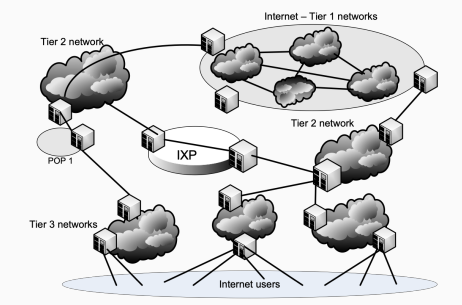
\includegraphics[scale=0.6]{images/network tiers.png}
            \caption{network tiers (nowadays an old model)}
            \label{fig:nettiers}
        \end{figure}
        
    \subsubsection{history}
        Over the time things changed and content-delivery network reshaped the definition of a network. At a certain point content providers had to deal with a growing demand of streaming services (because devices had become less expensive). That was a big problem because the network bandwidth was quite limited and content providers needed to guarantee the quality of their services (requesting more bandwidth). The main cause of this problem was the link connecting homes to the ISPs (called "last mile").
        
        Over years there has been a competition between national backbones (like Telecom Italia) and some big companies that created their own data centers and infrastructures.
        
        \FloatBarrier
        At the beginning, in fact, there where some national backbones operators that, thanks to some regional access providers and local access providers, brought Internet to costumers

        \begin{figure}[h!]
            \centering
            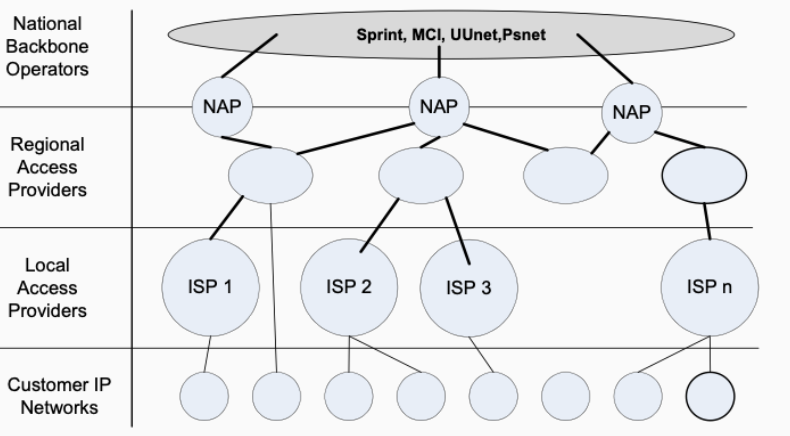
\includegraphics[scale=0.3]{images/providing structure 1.png}
            \caption{providing structure in 2007}
            \label{fig:nettiers}
        \end{figure}
        \FloatBarrier
        
        With the increased demand of services and bandwidth some hyper giants build their own structures and data centers everywhere and started providing their services.
        
        \FloatBarrier
        Nowadays the two entities works at the same time thanks to some Internet Exchange Points (IXP) that allows different ISP to exchange their Internet traffic each other.
        \begin{figure}[h!]
            \centering
            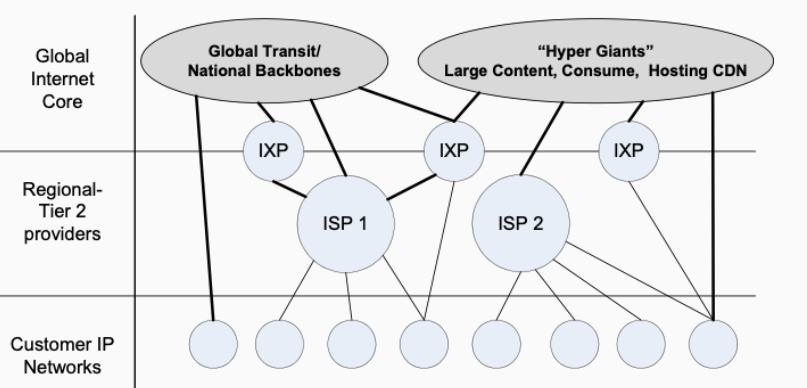
\includegraphics[scale=0.3]{images/providing structure 2.png}
            \caption{providing structure in 2009}
            \label{fig:nettiers}
        \end{figure}
        \FloatBarrier
        
        Google found another way of offering its service: it entered in some agreements with Telecom Italia to gets portion of Telecom Italia infrastructures to provide cloud services. In this way they didn't need to build new infrastructures spending more money.
        
        %Service provider is different form connectivity provider!
        
        
    \subsubsection{Characteristics}
        All modern data-centers shares some characteristics:
        
        Nowadays data center are structures with lots and lots of switches and routers (huge scale) that work with \textbf{high bandwidth} and with \textbf{very low round trip time}. From the point of view of the structure, they are quite homogeneous (they tries to have the same hardware [COTS]), with a regular topology and limited area occupations.
    
        However there are many aspects that can be changed:  the administrative domain, the routing, addressing and so on.
        % in some infrastructure there are paths that have the same costs that you can chose to use).
    
    
    \subsubsection{Requirements}
        In terms of requirements:
        \begin{itemize}
            \item Data centers work with lots of different connection flows. They must take care of both mice and elephant flows, it's need a low-latency user interaction.
            \item Data centers can work for a single and specific application (Google, Facebook, ...) or for some cloud service.
            \item Data centers works with two traffic directions:
            \begin{itemize}
                \item Outward, serving web pages to users
                \item Internal computation. Computation between data center is increasing more and more in relation with computation of user with data centers
            \end{itemize}
            \item Data centers often work with unpredictable workloads
        \end{itemize}
        
        
    \subsubsection{interconnection networks}
        A network is characterized by a common ensemble of elements that consists in:
        \begin{itemize}
            \item a set of nodes (processors, memory units, servers)
            \item links or communication channels
            \item a routing protocol used across nodes
            \item a flow control to menage congestions (usually in TCP level)
        \end{itemize}
        
        Switches are the components that receive data packs, identify the destination and uses routing tables to forward data packs until the destination. Thanks to them we can distinguish two network topologies:
        \begin{itemize}
            \item Static networks (direct connections between servers). Examples are: Bus, Hypercube, 2D-mesh and Torus topologies.
            \item Switched networks (switches are used to interconnect servers). Examples are crossbar and Omega switches
        \end{itemize}
        The topology will determine:
        \begin{itemize}
            \item the Network diameter
            \item the bisection width (if you cut the network at a certain point, is the minimum number of cuts to reach two halves)
        \end{itemize} 

        
    \subsubsection{Cloud interconnection networks}
        On top of servers there are some \textbf{aggregate switchers} that connect all servers. They can be optical or eletrical. Over them there is another layer of \textbf{core switches}.
        Ideally every server should be able to communicate with every other server with similar speed and latency.
        
        Yet Servers are largest amount of cost in a data center. So reducing it there will be a huge save of money.
        
        So the requirements for cloud interconnection are: Scalability, low cost, low-latency, high bandwidth and location transparent communication\footnote{Every server should be able to communicate with every other server with similar speed and latency}.
        
        
    \subsubsection{Conventional data center network}
        Every data center owner accord the design of it and the layers. In particular he can chose if working with layer 2 or layer 3.
        \begin{itemize}
            \item Playing with layer 2 allow working with fixed addressing and auto-configurations (much easier). However it has some limitations in the broadcast scale (ARP limitations)
            \item Playing with layer 3 guarantees more scalability through addressing and allow working with multipath routing (with equal costs). However it's more complex and do not guarantee migration without changing IP addresses
        \end{itemize}
        %We usually call POD (different from kubernetics) the layer 2.
        
        \FloatBarrier
        Data center looks as a giant switch that guarantee every connectivity (going from a server to another).
        Data center adopt the Clos topology that's base on  multiple stages. They are basically two butterfly networks that are inverted. It looks like a upside down fat tree.
        \begin{figure}[h!]
            \centering
            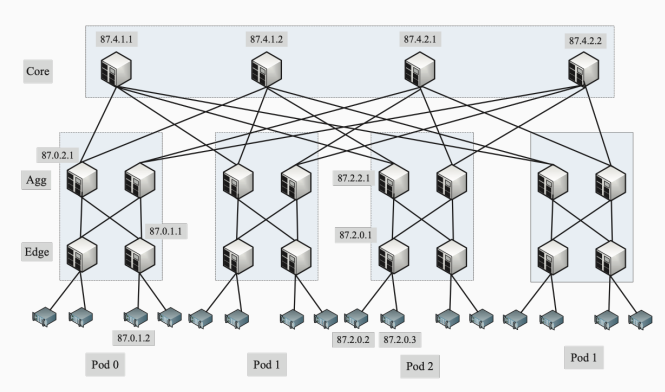
\includegraphics[scale=0.4]{images/clos topology.png}
            \caption{Clos topology}
            \label{fig:nettiers}
        \end{figure}
        \FloatBarrier
        
        Design principles:
        \begin{itemize}
            \item there are many of possible paths that cross exactly the same mount of links to go from one node to another
            \item the network can scale easily by changing some parameters
            \item multiple core switches
        \end{itemize}
        
        The main advantage of working with fat trees is that they are an optimal interconnection for large-scale clusters. In this cluster the servers are placed at the leafs, switches populate the root and the internal nodes of the tree. This is super regular and all switching elements of a fat-tree are identical.
        It's regular also in the number of elements: given the parameter $k$, you will have have $k$ pods; each pod has two layers; each layer has $\frac{k}{2}$ switches; each switch in the lower layer has connected to $k$ layers; every switch is connected to the aggregation layer. 
        
        Switches and pods are numbered and accessed by an IP address.
        
        There are some open issues to manage:
        \begin{itemize}
            \item There are different type of workloads with different requirements:
            \begin{itemize}
                \item Small flows (mice flows) requiring low-latency
                \item Large flows (elephant flows) requiring high-throughput
            \end{itemize}
            A datacenter needs a way of balancing them in order to provide to both of them a good service.
        
            \item Another issue is that TCP does not perform well in data center networks (we have to replace it with for example \textit{QUIC} or other networking protocols).
        \end{itemize}
        
        
        there are many equal costs path to go form one point to another. There are random allocated paths. The problem can be is that it doesn't care on resources occupation. May happens that if you have multiple elephant flow you may have collisions. If you have to elephant flows you have no problem. You can have collision also in the downward path. How do you menage flows within a data center network? There's research on this, quite advanced.
        
    \subsubsection{How to balance traffic flows}
        Assuming we want to go from the point S to the point D, there are many flows possible with equal cost path. Assuming that there's just one path down from each core switch:
        \begin{figure}[h!]
            \centering
            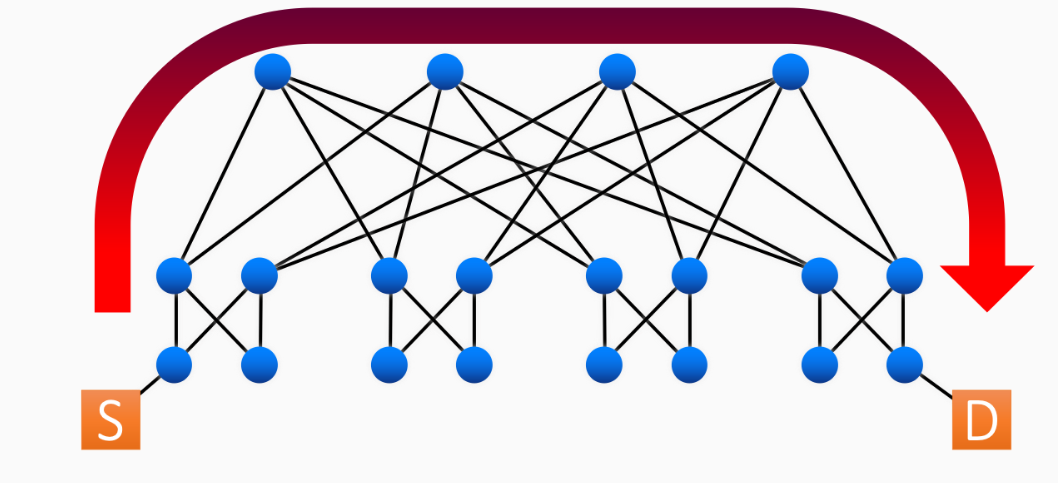
\includegraphics[scale=0.15]{images/trafficflow1.png}
        \end{figure}   
        
        The routing strategy to menage flows that is applied is \textbf{ECMP} (\textit{Equal-Cost Multi-Path}) that provides that paths are randomly allocated to flows (using hash of the flow).
        This routing strategy has the problem of not considering the limitation of available resources and can cause long lasting collision between elephant flows.
        
        To avoid this problem we can use Hedera, a scheduling technique that tries to detect elephant flows, computes non-conflicting paths and instructs switches to reroute traffic.
        
        There are many other possible solutions:
        \begin{itemize}
            \item Rerouting based on link utilization (but with the disadvantage of affecting mice flows)
            \item Rerouting based on switch queue occupancy, in particular removing elephant flows (that fill the most queues) and moving them away (but with the disadvantage of huge computation required)
            \item Spreading all packets uniformly (but with the disadvantage of more complicated TCP controls)
            \item Someone even proposed to change directly the TCP protocol
        \end{itemize}

    
    \subsection{Networking in virtualized environments}
        \FloatBarrier
        After creating multiple virtualized environments on a server (VMs, lightweight environments, containers), we need a sort of software bridge within the server that links their virtual network card to the virtual switch created by the OS.
        \begin{figure}[h!]
            \centering
            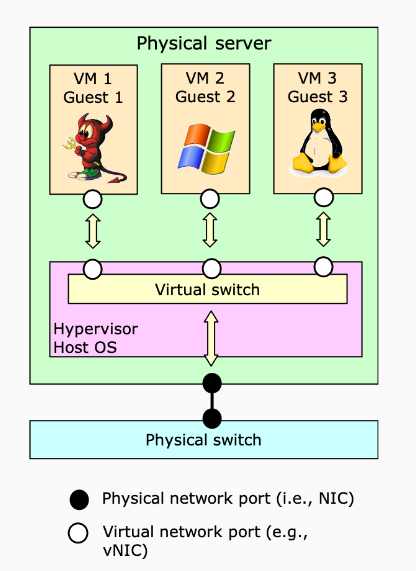
\includegraphics[scale=0.25]{images/virtualnet.png}
        \end{figure}
        \FloatBarrier
        
        From the point of networking, virtualization introduces additional complexity: in fact we need to deliver traffic from virtual to physical network (and vice versa) and between VMs/LXCs (within the same server).
        An additional requirement is to assign IP addresses to VMs/LXCs and provide advanced features such as load balancing, firewall ecc.
        
        In order to do this we need at first to provide Ethernet (L2) connectivity to VMs/containers and then to provide IP connectivity to them.

    
    \subsubsection{North/South and East/West communication on a single server}
        \FloatBarrier
        We can solve the problem presented above with at least three methods:
        \begin{itemize}
            \item Virtual (software) switch embedded in the OS
            \item In the NIC (using the physical network interface card and going back to the VM)
            \item In the external switch (getting out of the server, reaching the physical switch and the coming back)
        \end{itemize}   
        \begin{figure}[h!]
            \centering
            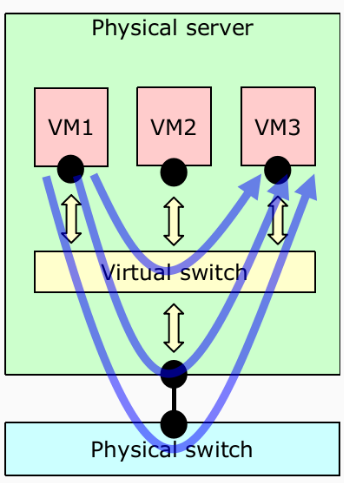
\includegraphics[scale=0.25]{images/virtserver.png}
        \end{figure}
        \FloatBarrier

        
        \myparagraph{Host-based switching}
            Historically the first solution ever used and the easiest one is \textbf{host-based switching} (or \textit{software bridge}). This solution works very well because the traffic is managed inside the server (high bandwidth) using some function given by the kernel without using the Internet layer (that has less capacity).
            One disadvantage is that it generates additional processing overhead and consumes CPU cycles. Another disadvantage is that it requires an additional component.
            Anyway this is the currently most common solution.
            
            Let's go deeper.
            
            The kernel is not a continuos process but it's triggered and reacts to events (event-based) that can be interrupts, system calls and whatever to interact.
            When a packet arrives a driver calls some functions of the kernel that menages packet. These function are called \textit{ETH Input} and they call \textit{IP Input} functions. These last function calls \textit{IP Forward} functions that understands where to sand packet by checking the routing table. 
            
            From a physical point of view, packets are moved by copying them from one VM in a space of memory reserved to the kernel and copied again in the second VM.
            
            A software bridge can be considered as an another function that is called to handle a packet on the layer 2. So a set of specific packets from virtual interfaces, instead of calling \textit{IP Input} functions, can go from \textit{ETH Input} functions to directly the Software bridge function at level 2.
            
            After that the bridge handles packets and calls the \textit{ETH Output} function which basically sands packets to a specific virtual interface of the machine.
            
            In addition, with software bridges you can apply policy directly in the virtual switch, intercepting the traffic before of other solutions.
            
            
        \myparagraph{Hairpin switching}
            The Hairpin switching use hardware that is already present (that has to be compatible).
    
            In particular packer are sanded to the physical switch and then received back in other VMs.
            
            It's slower then the previous one but don't use CPU cycles. Anyway This solution it's no longer used.
            

        \myparagraph{NIC switching}
            An intermediate solution is the NIC switching (intermediate also in terms of strengths and weaknesses). 
            
            In this solution we use some bridges called NICs in order to connect directly to the physical switch. These can be considered part of the network infrastructure because they are not controlled by the OS (and don't use the CPU capacity).
            
            In this way NICs avoid the problem about who controls edges switches.
            
            Another advantage is that, dedicating to NICs the job of transmitting packets, prevent DDoS attacks to affect these packets.
            
            In conclusion NICs gave the opportunity to researchers to  create smartNICs\footnote{A NIC with a processor and memory (like a GPU)}.
            

    \subsection{Software bridges in Linux}
        A software bridge provide intra-host connectivity to execution containers and handle IP addresses differently from the "official" IP model avoid the assignation of IP addresses to each network interface card (as opposed to the one IP address per NIC rule).
        
        \FloatBarrier
        A schema of basic bridging networking in Linux is the following:
        \begin{figure}[h!]
            \centering
            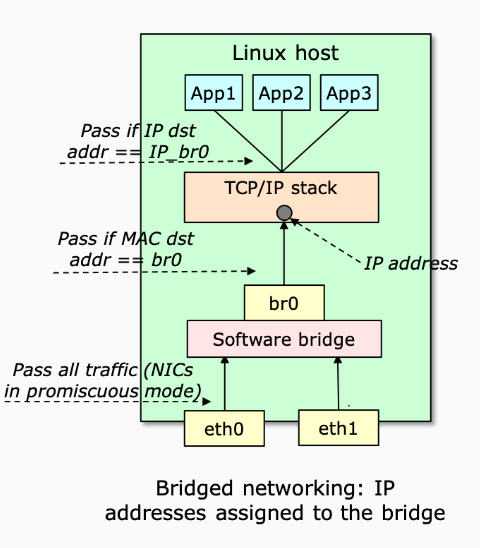
\includegraphics[scale=0.25]{images/bridgeschema.png}
        \end{figure}
        \FloatBarrier
        
        In order to avoid multiple IP addresses for each VM, the network interface card can be configured in a promiscuous mode. In this way every packet that is not intended for the machine MAC will be sand to the TCP/IP stack (crossing the internet interface transparently).
        
        Linux has three main types of software bridges:
        \begin{itemize}
            \item Linuxbridge
            \item Macvlan
            \item Open vSwitch
        \end{itemize}
    
    \myparagraph{Linuxbridge}
        Linuxbridge is the most common and simple one. It's a standard software provided by Linux that has everything that a physical switch needs; so it behaves like a traditional hardware switch (NICs has to be in promiscuous mode).
    
    \myparagraph{Macvlan}
    
        We define \textit{vlan} a broadcast domain (group) of ports used to partition lan in order to have a level 2 separation and isolation.
        
        Macvlan implements a VLAN-like behavior by using MAC addresses instead of tags. Macvlans look like a L2 interface with a personal and distinct MAC address (they can have a distinct IP address too).
        
        Macvlan support some operating modes:
        \begin{itemize}
            \item Private: makes a VLAN-like behavior; two macvlan belonging to different broadcast domains communicate thanks to routing.
            \item Virtual Ethernet Port Aggregator (VEPA) - Default mode: allows MAC A to talk with MAC B only if the traffic comes from the external world (so a switching element is required)
            \item Bridge: macvlan driver acts like a bridge; it's simple and fast
            \item Pass-through: it basically works by assigning directly cards to VMs (not much used)
        \end{itemize}
  
        
        \subsubsection{Open vSwitch}
        Open vSwitch is a software implementation of a virtual multilayer network switch that you can configure by using protocol used with real switches (so you can directly decide what to do with packets). It's much more complicated.
    
    
    \subsection{Single server: complex services}
        From a high level point of view, there are still some problem in attaching VMs to a virtual switch:
        \begin{itemize}
            \item what are the IP addresses provided to VMs? How to assign them?
            \item More network services may be required besides setting up bridge
            \item How to provide multi-tenancy? (multiple isolated environments that can communicate each other dedicated to multiple people in the same server or in different servers too). Tenants than can require additional networking services
            \item A NAT and a routing table is required too (connectivity is much complex than a single switch).
            \item How to manage TCP/IP stack?
        \end{itemize}

    \subsubsection{IP address assignment}
        The first problem to solve is how to assign IP addresses. There are different possible ways of doing it:
        
        \begin{itemize}
            \item The first option is \textbf{direct routing} that uses some IP addresses known by the physical network. This solution can be implemented in two ways:
            \FloatBarrier
            \begin{itemize}
                \item \textbf{Bridged mode}: VMs ask for IP addresses directly to the physical network. So VMs are directly attached to a vSwitch. In other words VMs rely on a upstream DHCP server to receive an IP address
                \item \textbf{Routed mode}: in this mode VMs ask for an IP to a vSwitch linked to a vDHCP server; so the router must know that to reach VMs it has to reach a vSwitch before
            \end{itemize}
            
            \begin{figure}[h!]
                \centering
                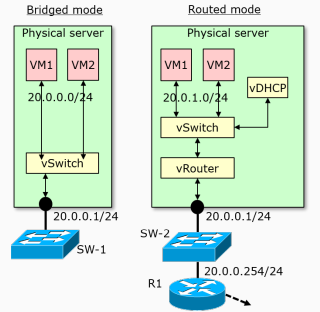
\includegraphics[scale=0.55]{images/IP ass.png}
            \end{figure}
            \FloatBarrier
            
            Pros of direct routing is that no NATting service is require because inbound and outbound connections are the same.
            
            Anyway it has many problems: how many IP addresses can be assigned? Than it will require the coordination of the network manager too. These cons made this solution not really the most used.
            
            Coordination with the network manager is required because we can't configure by ourselves router tables (that have information about directly attached network and other routers that can be used to reach networks not directly attached)
            
            \item The second option is \textbf{NATTed mode} that uses a vDHCP service to provide a private IP addresses to the VM (as it was a private network). vSwitch and vDHCP can be managed by the tenet.
            
            The connection to the Internet is than allowed by a NAT service. In fact there's a vNAT that changes private IPs (10.0.0.0) into Internet traffic (20.0.0.0).
            
            An advantage with this method is that no coordination with the network manager is required.
            
            A cons is that VMs are reached with different IPs (private or public) depending if the sender is inside or outside the private network.
            
            This model is used by Docker uses this model.
        \end{itemize}
        
        
    \subsubsection{Providing feature-rich network connectivity}

        To connect a VM to the physical infrastructure additional network services may be required (Router, NAT and DHCP for using private addresses). All these services are usually provided by by Linux itself or can be installed.
        
        In Docker there's some kind of DHCP service that works with the same concept but without using that exact protocol.
        
        
    \subsubsection{multi-tenancy}
        \FloatBarrier
        The solution for supporting multiple tenents on a physical server is to use as many vSwitch and vRouters as many tenets I need.
        
        This approach is preferred to vLANs because it is completely software based and it's easier to configure and manage rather than vLANs.
        \begin{figure}[h!]
            \centering
            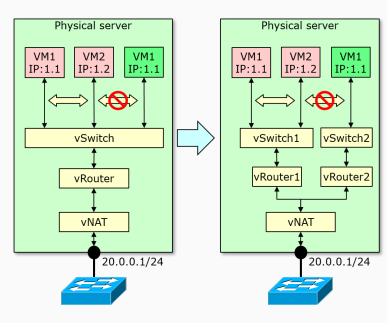
\includegraphics[scale=0.55]{images/multi tenancy.png}
        \end{figure}
        \FloatBarrier
        
        
        
    \subsubsection{Tenant-defined network services}
        \FloatBarrier
        A single tenet may want pretty complex services like having multiple machines but exposing just one to the vSwitch through a L7 firewall (in order to defend the VM and to filter possible queries); So the tenant can create more complex service on its own. It can use Linux provided functionality or functionality provided by some installations.
        \begin{figure}[h!]
            \centering
            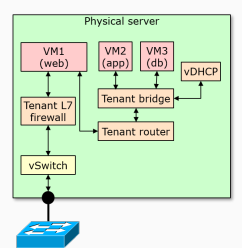
\includegraphics[scale=0.4]{images/tenant services.png}
        \end{figure}
        \FloatBarrier
        
        
    \subsubsection{Co-existence of virtual services and host applications}
        \FloatBarrier
        Within the server we have a TCP/IP stack (used with some applications that run on the server) that need to coexist with VMs.
        \begin{figure}[h!]
            \centering
            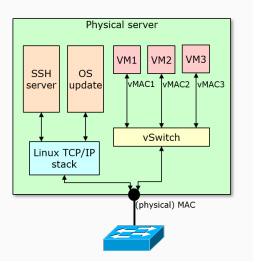
\includegraphics[scale=0.55]{images/TCP IP stack.png}
        \end{figure}
        \FloatBarrier
        
        In particular in order to distinguish inbound traffic toward VMs the physical interface on the server use hardware filtering: a packet that arrives with a MAC address not recognized will be dropped.
        
        In a bridged mode, MAC addresses will be different from the physical one, so we need to configure the physical card to be in promiscuous mode. This is not needed if using a vRouter NAT.
        Than inbound traffic is recognized by using different MAC addresses (otherwise we can use ports or use some intelligent software).
        
    
    \subsubsection{vNIC}
        Supposing that a VM want to send a packet, how to understand if it's for the Internet or for another VM?
    
        A \textbf{vNIC} is a device driver that connects VMs with the Linux IP stack and with the vSwitch (it can be implemented simply as a virtual ethernet interface).
        
        It's a network interface that is attached in the namespace where VMs are and links the root namespace (by facts it runs in the Linux kernel). 
        
        When the vNIC receives a packet it detects the destination of it. If it's the Internet, it sands it to the Linux IP forwarding module (technically to the default gateway). After that the kernel will manage it by looking to routing tables and using ARP protocol.
        
        \myparagraph{Practical example}
            Let's assume that the VM1 wants to sand a packet to the Internet. The packet that exits the VM has a source address 10.0.0.1 (MAC of the VM) and a destination address 8.8.8.8 (that's the MAC of the vNIC, learnt by a broadcast request) and it has to go via 10.0.0.254. This packet gets to the vSwitch that does a filtering forwarding. The packet is than sand to the vNIC that look to the destination: if it's not for the vNIC it will be sanded to the forwarding module of the kernel that will use a routing table and the IP address as a gateway.
        
        
    \subsection{DC-wide services}
    
        We want now to connect VMs across different physical servers. Thinking wide, when moving from a single server to a datacenter, the problems to solve are the same of VMs but with a different scale (datacenters can include thousand of servers): IP address assignments, supporting multiple tenants and so on.
        
        \FloatBarrier
        Let's distinguish two point of view:
        \begin{itemize}
            \item The tenet wants to deploy its virtual service ignoring the physical infrastructure (number of servers and connection between them); in fact VMs can be on different servers;
            \item The Cloud manager has to build the infrastructure that the Tenet uses.;
        \end{itemize}
        \begin{figure}[h!]
            \centering
            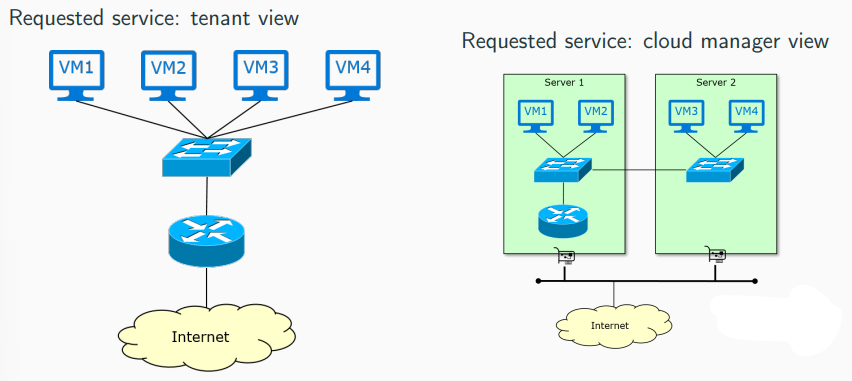
\includegraphics[scale=0.55]{images/point of views.png}
        \end{figure}
        \FloatBarrier

    \subsubsection{Providing L2 connectivity to tenant services across DC}
    
        Let's assume that a costumer wants to have a L2 network among all its services (VMs). In order to allow that, the Cloud manager needs to create a tunnel between switches of servers.
        
        
        
        L2 connectivity to services of tenents across different machines or L3 connectivity. This is a decision of the customer, depending on what he wants. We want all VMs connected as i would have a L2 connection. We need to create a tunnel between switches of servers.
        From the point of view of the cloud manager we have multiple servers with different VMs over them.
        In a physical environment i would have some machine and a switch. In virtual world is different. 
            
        \FloatBarrier
        Let's assume that a tenant has VM1, VM2, VM3 and VM4 and that he wants them to be connected as they was in a bridged network (it doesn't know they are in different servers).
        \begin{figure}[h!]
            \centering
            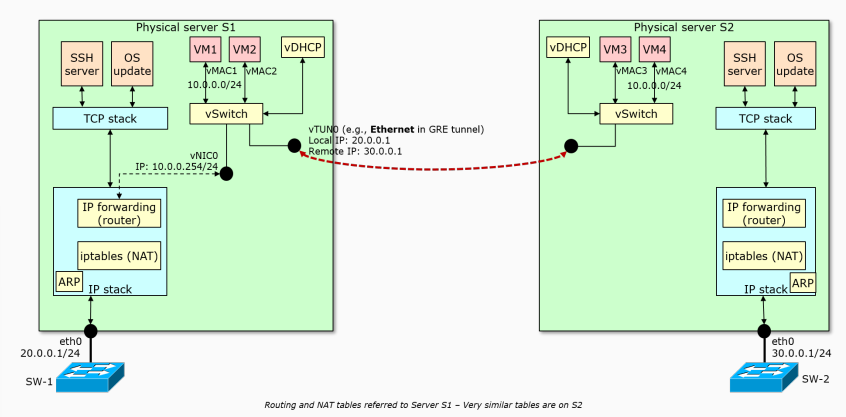
\includegraphics[scale=0.5]{images/example of tunneling.png}
        \end{figure}
        \FloatBarrier
        
        In real world different machines could be connected by using two switches connected with an ethernet cable.
        
        The same happens in virtualized world: the Cloud manager creates a tunnel from a \textbf{vTUN0} interface (that has the same characteristics of an internet interface). The VTUN0 uses the \textbf{GRE protocol}; in particular it encapsulates frames or packets, add some small in-layers and another IP header with the localIP (source) and the remoteIP (destination).
        As result, we connected two machines with a L2 connection.
        
        With this connection the vNIC in the second server is no longer required: packets sanded from VM3 and VM4 can use pass trough the vTUN0 and use the vNIC0 of the first server.
        
        
    \subsubsection{Providing L3 connectivity to tenant services across DC}
        If a customer asks for a L3 connectivity without caring of the L2 one (neither about IP addresses), there are two possible working modes:
        \begin{itemize}
            \item tunneling
            \item direct routing
        \end{itemize}
        
        \FloatBarrier
        In \textbf{tunneling} a tunnel directly attached to the IP forwarding router is used. This tunnel will use the \textbf{IP in GRE} protocol; so in the encapsulation phase the IP packet will be put in another IP packet (so the tunnel needs to have a dedicated IP address).
        The first IP header will be than removed on the server 2.
        \begin{figure}[h!]
            \centering
            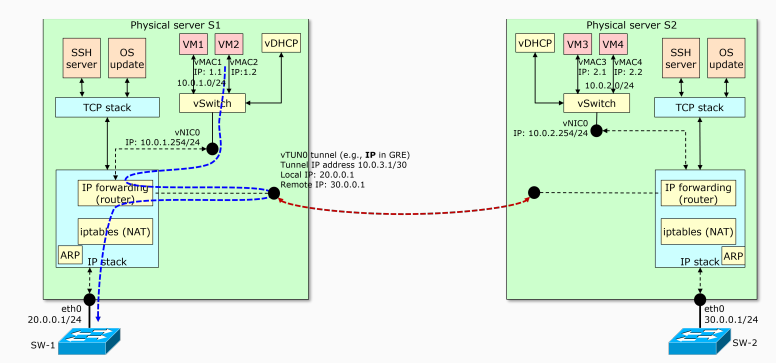
\includegraphics[scale=0.5]{images/tunneling.png}
        \end{figure}
        \FloatBarrier
        
        A possible problem is that when doing encapsulation the packet size is increased (because of the addition of another header). This could be a problem if the packet have already reach the maximum size. The solution is fragmentation which however adds some overhead.
        
        \FloatBarrier
        Otherwise, if fragmentation is not acceptable, \textbf{direct routing} is the last solution. The packet will be sand outside of the S1 and trough a router will be received by the second switch that will sand to the S2.
        \begin{figure}[h!]
            \centering
            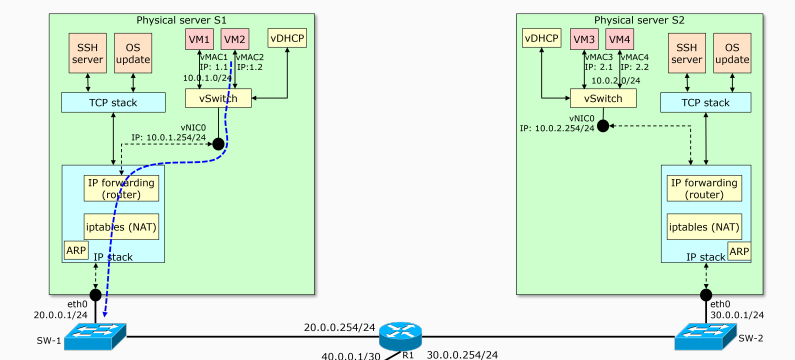
\includegraphics[scale=0.5]{images/direct routing.png}
        \end{figure}
        \FloatBarrier
        
        Summarizing:
        \begin{itemize}
            \item Overlay (tunneling)
            \begin{itemize}
                \item no interaction with the infrastructure is required
                \item adds some overhead (logical channels over physical ones)
            \end{itemize}
            \item Direct routing
            \begin{itemize}
                \item requires the collaboration of the infrastructure provider
                \item 
            \end{itemize}
        \end{itemize}